\documentclass[english, 12pt, a4paper, sci, a-1b, online]{aaltothesis}

\usepackage[numbers]{natbib}
\usepackage{graphicx}
\usepackage[most]{tcolorbox}
\usepackage{amsmath, amsthm}
\usepackage{unicode-math}
\setmathfont{texgyrepagella-math.otf}

\usepackage{tkz-graph}
\usepackage{tikz}
\usetikzlibrary{calc}
\usetikzlibrary{arrows.meta}

\usepackage{minted}
\usemintedstyle{friendly}
\setmonofont{DejaVu Sans Mono}
\setminted{fontsize=\footnotesize, autogobble}
\newcommand\icoq[1]{\mintinline{Coq}{#1}}
% horrible hack to hide pygment's complaints about unicode
\AtBeginEnvironment{minted}{\dontdofcolorbox}
\def\dontdofcolorbox{\renewcommand\fcolorbox[4][]{##4}}

\usepackage{graphicx}
\graphicspath{{./images/}}

\degreeprogram{Computer, Communication and Information Sciences}
\major{Computer Science}
\code{SCI3042}

\univdegree{MSc}
\thesisauthor{Joonatan Saarhelo}
\thesistitle{Fast and Correct Round Elimination}
\place{Espoo}
\date{2021}

\supervisor{Prof.\ Jukka Suomela}
%\advisor{}

%% \uselogo{aaltoRed|aaltoBlue|aaltoYellow|aaltoGray|aaltoGrayScale}{?|!|''}
\uselogo{aaltoRed}{''}

\keywords{For keywords choose\spc{}concepts that are\spc{}central to your\spc{}thesis}

\thesisabstract{
Your abstract in English. Cannot contain special characters, linebreak or paragraph
break characters as it is written into the metadata.
}

%% Copyright text. Copyright of a work is with the creator/author of the work
%% regardless of whether the copyright mark is explicitly in the work or not.
%% You may, if you wish, publish your work under a Creative Commons license (see
%% creaticecommons.org), in which case the license text must be visible in the
%% work. Write here the copyright text you want. It is written into the metadata
%% of the pdf file as well.

\copyrighttext{Copyright \noexpand\copyright\ \number\year\ \ThesisAuthor}
{Copyright \textcopyright{} \number\year{} \ThesisAuthor}

\begin{document}

\makecoverpage{}

\makecopyrightpage{}

\begin{abstractpage}[english]
  \abstracttext{}
\end{abstractpage}

\newpage

\thesistitle{Nopea ja virheetön kierroseliminaatio}
\keywords{Vastus, resistanssi, lämpötila}

\begin{abstractpage}[finnish]
  Tiivistelmässä on lyhyt selvitys
  kirjoituksen tärkeimmästä sisällöstä: mitä ja miten on tutkittu,
  sekä mitä tuloksia on saatu. 
\end{abstractpage}

\thesistableofcontents{}


\mysection{Symbols and abbreviations}

\newtheorem{theorem}{Theorem}[section]
\newtheorem{lemma}{Lemma}[section]
\newtheorem{corollary}{Corollary}[theorem]

\newcommand{\reline}[1]{\textbf{#1}}

\tikzstyle{active} = [draw, thick, circle, fill=white, minimum size=1.5em]
\tikzstyle{passive} = [draw, thick, circle, fill=darkgray, text=white, minimum size=1.5em]

\subsection*{Symbols}

\begin{tabular}{ll}
\end{tabular}

\subsection*{Abbreviations}

\begin{tabular}{ll}
RE         & round elimination
\end{tabular}

\cleardoublepage{}
\section{Introduction}

%% Leave page number of the first page empty
\thispagestyle{empty}

\clearpage
\section{Background}

Today's world is filled with software and most of it doesn't always work as intended.

Testing can be used to verify the correctness of programs that take a small finite amount of different inputs.

Fuzzing means running software against computer-generated inputs. AFL-fuzz~\cite{AFL} is a highly optimized fuzzer that monitors program execution in order to find inputs that trigger previously unexplored execution paths. It has been used to find intricate bugs even in complex software.

One crash that I have found by fuzzing was caused by code that assumed that one can compute the absolute value of any machine integer. However, taking the absolute value of the smallest representable integer (for example -128 for 8-bit integers) leads to undefined behaviour because there is always one negative integer more than there are positive integers in two's complement.

Fuzzing is best at finding crashes but it can be used to find incorrect behaviour by writing a program that crashes whenever an incorrect output is produced. However it is only effective if outputs can be computed and checked very quickly.

SAT-solvers can be used to find cases where algorithms fail on finite but relatively large inputs and even perform an exhaustive search to show that no such cases exist.

Formal proof can establish correctness of algorithms even for arbitrarily large inputs. Proofs are completely unaffected by how expensive it is to compute or check outputs. Unfortunately, theories that are simple to state can have very large proofs.

Perharps the most notable example is Thomas Hales' proof of the Kepler conjecture. The Kepler conjecture states that there is no way of packing spheres more densely than the cannoball packing, in which the spheres are arranged in hexagonally packed layers and those layers are stacked on top of each other. In 1831, Gauss proved a proposition about polynomials that can be used to show that a variant of the aforementioned packing is the densest possible lattice packing of spheres.~\cite{dichteste} However, before Hales' proof the possibility of a denser irregular packing wasn't ruled out.

A proof consisting of a computer program that solves linear programming problems and hundreds of pages of notes was completed in 1998. After four years of inspecting the proof, a panel of twelve referees announced that they couldn't be completely certain if the computer calculations were correct. That prompted Hales to start the Flyspeck project, which completed a complete formal proof of the Kepler conjecture in 2014.

Pitäisiköhän tästä kertoa enemmän?

TODO cite

\subsection{History of computer-aided mathematics}

TODO This will maybe be just part of the introduction?

\section{Locally Checkable Labeling}

Locally checkable labeling (LCL) is a family of graph problems in which one has to assign colors to edges or vertices, satisfying some locally checkable condition.~\cite{LCL}

Locally checkable means that a solution can be checked by checking fixed size neighborhoods. For example, to verify that vertices are properly colored, one just has to look at the neighbors of each vertex and check that no neighbor has the same color.

When every vertex has at most $\Delta$ outgoing edges, an LCL-problem can be given as a finite set of allowed neighborhoods, where $\Delta$ is the maximum degree of the graph.

\newcommand\tick{\fill[scale=0.6, color=black!40!green](0,.35) -- (.25,0) -- (1,.7) -- (.25,.15) -- cycle;}
\newcommand\cross{\draw[scale=0.3, very thick, color=red] (0,0) -- (1, 1) {} (0, 1) -- (1, 0) {};}

\begin{figure}[h]
\centering
\begin{tikzpicture}[line width=1pt]
  \foreach \i/\a/\b/\c/\ok in {0/-latex/latex-/latex-/\tick, 1/-latex/-latex/latex-/\tick, 2/-latex/-latex/-latex/\tick, 3/latex-/latex-/latex-/\cross}
  {
    \tikzset{xshift={\i * 7em}}
    \node [active] at (0,0) (center) {};
    \draw [\a] (center) -- (-90:1);
    \draw [\b] (center) -- (30:1);
    \draw [\c] (center) -- (150:1);
    \tikzset{xshift=1.4em, yshift=-1.8em}
    \ok
  }

  \tikzset{yshift=5em}
  \foreach \i/\a/\b/\ok in {0/-latex/latex-/\tick, 1/-latex/-latex/\tick, 3/latex-/latex-/\cross}
  {
    \tikzset{xshift={\i * 7em}}
    \node [active] at (0,0) (center) {};
    \draw [\a] (center) -- (-1,0);
    \draw [\b] (center) -- (1,0);
    \tikzset{xshift=1.4em, yshift=-1.8em}
    \ok
  }

  \tikzset{yshift=5em}
  \foreach \i/\a/\ok in {0/-latex/\tick, 3/latex-/\cross}
  {
    \tikzset{xshift={\i * 7em}}
    \node [active] at (0,0) (center) {};
    \draw [\a] (center) -- (-1,0);
    \tikzset{xshift=1.4em, yshift=-1.8em}
    \ok
  }
\end{tikzpicture}
\caption{An exhaustive list of neighborhoods for checking sinkless orientation in a graph with maximum degree three.}
\end{figure}

I will use \emph{sinkless orientation} as running example in this paper. It is the problem of selecting a direction for each edge so that no vertex has only incoming edges. To check sinkless orientation, it is suffices to see the neighboring edges. There are other problems that require seeing a larger neighborhood, such as distance-2 coloring, the problem of choosing different colors for every pair of vertices the shortest distance of which is two.

\newcommand\samplegraph
{
  \node [active] at (0,0) (a) {};
  \node [active] at (1,0) (b) {};
  \node [active] at (2,0) (c) {};
  \node [active] at (1.5,1) (d) {};
}

\begin{figure}[h]
\centering
\begin{tikzpicture}[line width=1pt]
  \samplegraph
  \draw (a) -- (b) -- (c) -- (d) -- (b);

  \tikzset{xshift=10em}
  \samplegraph
  \draw [-latex] (a) -- (b);
  \draw [-latex] (b) -- (c);
  \draw [-latex] (c) -- (d);
  \draw [-latex] (d) -- (b);
\end{tikzpicture}
\caption{An undirected and the unique solution to sinkless orientation in it.}
\end{figure}

\subsection{Round Elimination problems}

\emph{Biregular graphs} are graphs that have properly two-colored vertices and where the degree of each class of vertices is constant. Round Elimination operates on edge coloring LCL-problems in biregular graphs that can be checked by only checking the nearest edges' colors. I call this kind of problem a \emph{Round elimination problem} or RE problem.

Sinkless orientation is not such a problem. To begin with, edge orientation is not a color. However, there is an isomorphism between the solutions our sinkless orientation problem and the solutions of an RE problem. But first, I will present a simple way of representing RE problems.

In round elimination, one of the classes of the biregular graph is called the \emph{active side} and the other the \emph{passive side}. The active side nodes are active in the sense that they are the computers in a network that have to choose the colors of their neighboring edges.

Since each neighborhood can only see a vertex and a number of edges, we can simply list all multisets of edge colors allowed. They are called \emph{configurations} and are denoted with square brackets in this thesis. There are two sets of configurations, the configurations around active nodes, $A$, and the ones around passive nodes, $P$.

An RE problem can be represented as sets $A$ and $P$. The symbols in the configurations are from an alphabet $\Sigma$.

\subsection{Conversion from LCL}

I will now show how to represent sinkless orientation for RE. Each vertex in the original graph corresponds to an active vertex in the RE graph. Edges correspond to passive vertices. We can describe the directions of edges by coloring the RE graph's edges with I (for incoming) and O (for outgoing).

\begin{figure}[h]
\centering
\begin{tikzpicture}[line width=1pt]
  \node [active] at (5, 0) (center') {};
  \node [active] at (0, 0) (center) {};
  \foreach \a/\cl/\el/\arrow in {0/O/I/-latex, 120/O/I/-latex, 240/I/O/latex-}
  {
    \node [active] at (\a+18:1.4) (A){};
    \draw [\arrow] (center) -- (A)
    coordinate[near start] (tail)
    coordinate[near end] (head);

    \ifnum\a=240
      \node [passive, label=right:{passive}] at ($ (\a+18:1.5) + (center') $) (P) {};
      \node [active, label=right:{active}] at ($ (\a+18:3) + (center') $) (A') {};
    \fi
    \node [passive] at ($ (\a+18:1.5) + (center') $) (P) {};
    \node [active] at ($ (\a+18:3) + (center') $) (A') {};

    \draw (center') -- (P) node[midway, sloped, below] (CtoP) {\cl};
    \draw (P) -- (A') node[midway, sloped, below] (PtoA) {\el};
    \draw [dotted] \foreach \da in {-60, 60} {
      (A) -- ($ (A) + (\a+18+\da:0.8) $)
      (A') -- ($ (A') + (\a+18+\da:1) $)
    };
  };
  \draw [dashed, stealth-stealth, shorten <=0.6ex, shorten >=0.5ex] (tail) to[bend left=10] (CtoP);
  \draw [dashed, stealth-stealth, shorten <=0.5ex, shorten >=0.5ex] (head) to[bend left=10] (PtoA);
\end{tikzpicture}
\caption{Correspondence between solutions in round elimination graph and original graph}
\end{figure}

The active side's rule lists all the valid neighborhoods. The passive side's rule ensures that each edge is incoming on one end and outgoing on the other; otherwise there could be edges with an arrowhead on both sides.

\begin{align*}
\Sigma &= \{I, O\} \\
A &= \{[I, I, O], [I, O, O], [O, O, O]\} \\
P &= \{[I, O]\}
\end{align*}

The cases of sinkless orientation that deal with nodes of lower degree can be disregarded, since the active nodes in the biregular graph all have the same degree. (TODO but didn't we discover that we can do RE in non-regular graphs?)

TODO generalizing the conversion

\section{Round Elimination}

Brandt et al.~\cite{speedup} introduced round elimination in 2019. It is a procedure that takes a round elimination problem $\Pi_0$ and outputs a new problem $\Pi_1$. It has interpretations in various models of distributed computing. As the name suggests, $\Pi_1$ can generally be solved one round faster than $\Pi_0$.

While $\Pi_0$ assigns a color to each edge, $\Pi_1$ assigns a set of colors each edge. That set contains the colors that the edge could have in a solution to $\Pi_0$. There is uncertainty because in one round less some information that affects the solution of $\Pi_0$ is out of reach.

\subsection{Lines}

Dennis Olivetti~\cite{RE} wrote an implementation of round elimination called Round Eliminator. Round Elimination has been used to prove bounds on time complexity for various problems in the LOCAL model~\cite{tc1, tc2, tc3}.

In Round Eliminator, problems are represented as \emph{lines}. Lines are a kind of shorthand notation that compresses multiple configurations into one line. Each line is a multiset of sets and represents or \emph{generates} all the configurations obtained by choosing one color from each set.~\cite{RE}

For example, the line \reline{IO IO O} generates the configurations $[I, O, O]$, $[I, I, O]$ and $[O, O, O]$. ($[O, I, O]$ is the same as $[I, O, O]$, since lines and configurations are unordered.)

\begin{figure}[h]
  \centering
  \begin{tcolorbox}[width=.22\textwidth, nobeforeafter, title=active side]
  IO IO O
  \end{tcolorbox}
  \begin{tcolorbox}[width=.22\textwidth, nobeforeafter, title=passive side]
  I O
  \end{tcolorbox}
  \caption{Sinkless orientation in Round Eliminator's shorthand}
\end{figure}

\subsection{Formal definition}
The configurations of $\Pi_1$ have the exact same shape as lines of $\Pi_0$: multisets of nonempty sets of symbols from $\Pi_0$'s alphabet, so it is convenient to talk about them as lines. I will call $\Pi_0$'s alphabet, active side and passive side $\Sigma_0$, $A_0$ and $P_{0}$ respectively and use the same notation to refer to $\Pi_{1}$'s components

The definition of RE from Distributed Algorithms 2020~\cite{DA2020} rephrased in terms of lines:
\begin{itemize}
  \item $\Sigma_1$ is the powerset of $\Sigma_0$ minus the empty set.
  \item $A_{1}$ consists of all configurations that only generate configurations present in $P_{0}$.
  \item $P_1$ consists of all configurations that generate at least one configuration from $A_0$.
\end{itemize}

\subsection{Interpretation in the port numbering model}

In this section I'll show that the round elimination produces a problem that can be solved exactly one round faster than its predecessor in the port numbering model. The port numbering model is the weakest of a number of of models of distributed computing. The proof in the port numbering model has been used to show that the same property holds in stronger models. (TODO cite an example)

\subsubsection{The port numbering model}

In the port numbering model, each vertex runs the same program and must produce part of a solution to a problem defined on its graph. The problem need not be locally checkable and the graph does not need to be a tree but this thesis is about round elimination problems, so everything documented here has that shape.

Computation proceeds in a series of rounds. In each round, vertices send a message to each of their neighbors. Then all vertices receive the messages simultaneously. Finally, each vertex can either output its part of the solution and stop, or continue to the next round. Before, after and between these steps, the nodes get to compute as much as they want. This process repeats until all vertices have chosen their output.

However, everything stated in the previous paragraphs applies equally well to the LOCAL model for example. The defining characteristic of the port numbering model is that the only thing each vertex knows is that it is connected to its $n$ neighbors via ports numbered $1$ to $n$.

Formally, we can define a graph in the port numbering model as a set of connections between ports.
\begin{align*}
  \text{Port} = \text{Vertex} \times \mathbb{N} \\
  \text{Connection} = \{Port, Port\}
\end{align*}
Every port must be connected to only one other port. If a node's port $n$ is connected, ports $1$ to $n-1$ must be connected as well.

An algorithm in the port numbering model can be expressed as three functions.
\begin{align*}
  \text{send} &: \Pi_{n : \mathbb{N}}~\text{State} \to \text{Message}^n \\
  \text{recv} &: \Pi_{n : \mathbb{N}}~\text{Message}^n \to \text{State} \to \text{State} \\
  \text{result} &: \text{State} \to \text{Output} + 1
\end{align*}
The first one computes what messages to send based on the state the node is in; the second how a node's state changes when it receives its neighbors' messages. The first message in the tuple produced by $\text{send}$ is sent to port 1, the second to port 2 etc. Likewise, the first message in the tuple passed into $\text{recv}$ is the one received from port 1. Finally, the function called $\text{result}$ computes a node's output if it has stopped and returns unit otherwise. (The notation $\text{Output} + 1$ means $\text{Output}$ or unit. The one stands for a type that is inhabited by only one value.)

None that $\text{send}$ and $\text{recv}$ may behave differently based on the number of ports. In fact, they have to because $\text{send}$ must produce a tuple of messages of the correct length. The number of ports, $n$ cannot be a normal parameter, as the type of the function depends on its value. For an in-depth discussion of the $\Pi$ notation see Section~\ref{dependent} (Dependent types).

An $r$-round solvable problem is a problem for which there exists an algorithm that gives the correct output after $r$ rounds. It is easier to prove that round elimination works in the port numbering model by adopting a different perspective.

\begin{lemma}
  A problem is $r$-round solvable in the port numbering model if and only if each vertex can produce a correct output by looking at its $r$-neighborhood.
\end{lemma}
Here $r$-neighborhood refers to the subgraph containing vertices and edges at most $r$ edges away.

The $r$-neighborhood is sufficiently large, as information from further away cannot be seen in $r$ rounds. Every vertex can gather its $r$-neighborhood can be constructed in $r$ rounds, so it isn't too much information either.

The gathering process works as follows: In every round, every vertex sends everything it knows to its neighbors. TODO

\subsubsection{Round elimination in the port numbering model}

Suppose there is an algorithm $G_0$ that looks at an $r$-neighborhood and solves the round elimination problem $\Pi_0$. Let us construct an algorithm $G_1$ that looks at an $(r-1)$-neighborhood in a graph that is the same as the graph $G_0$ operates on but the active nodes are passive and vice versa.

Suppose that $G_1$ is run on some vertex $v$. For each neighboring vertex $n$, $G_1$ computes all possible $r$-neighborhoods centered around $n$. $G_1$ then runs $G_0$ on each of the neighborhoods, noting the color $G_0$ assigns to the edge $\{v, n\}$. $G_1$ assigns the union of all those colors to $\{v, n\}$.

TODO $r > 0$ and $r$ must be small enough that blind spots could all be full size.

\begin{lemma}
  $G_1$ solves $\Pi_1$, the result of running round elimination on $\Pi_0$.
\end{lemma}
\begin{proof}
  It suffices to show that $G_1$'s solutions satisfy $\Pi_1$'s active and passive side rule.

  All the edge colors surrounding a passive node are computed from the same part of the graph but with different blind spots. Since $G_0$ is run  with all possible values in the blind spots, there is a run where the blind spot has the same values as it does in reality. Thus each edge's set contains the color that $G_0$ would assign to that edge. Because $G_0$ solves $\Pi_0$, $A_0$ must contain a configuration with those colors. Therefore $P_1$ is satisfied, as all the passive nodes' surrounding edges generate a configuration from $A_0$.

  The edges $e_1, e_2, \ldots$ surrounding an active node are computed from neighborhoods whose blind spots are completely disjoint since the graph is a tree. Suppose the edges's colors generate some configuration $[a_1, a_2, \ldots]$ that is not in $P_0$. Then w.l.o.g.\ there exist some values for the blind spots such that $G_0$ colors $e_1$ with $a_1$, $e_2$ with $a_2$, etc. Because the blind spots are disjoint, it is possible to set them all to those specific values at the same time, which results in a graph where $G_0$ colors the edges around a passive node with a set of colors that isn't found in $P_0$ which is a contradiction, as we assumed that $G_0$ solves $\Pi_0$. Thus we know that the colorings of active nodes only generate configurations that are in $P_0$.
\end{proof}

\begin{lemma}
  $\Pi_1$ can be solved at least one round faster than $\Pi_0$.
\end{lemma}
\begin{proof}
  Suppose that $G_0$ is the fastest possible algorithm that solves $\Pi_0$. $G_1$ solves $\Pi_1$ one round faster than that.
\end{proof}

\begin{lemma}
  $\Pi_1$ can be solved at most one round faster than $\Pi_0$.
\end{lemma}
\begin{proof}
  If there is an algorithm $G_1$ that solves $\Pi_1$ in less than $r-1$ rounds, it is possible to solve $\Pi_0$ in less than $r$ rounds: run $G_1$ on all passive nodes and send the resulting edge colors to the neighboring active nodes. The definition of $P_1$ guarantees that each active node is able to pick a configuration that is in $A_0$ from the edge colors around it. The definition of $A_1$ guarantees that the passive rule is satisfied no matter what color the active nodes pick.

  But we assumed that the fastest algorithm solves $\Pi_0$ in $r$ rounds, so the assumption that $\Pi_1$ can be solved in less than $r-1$ rounds must be false.
\end{proof}

I have shown that $\Pi_1$ can be solved at least one round faster and at most one round faster than $\Pi_0$, so clearly it can be solved exactly one round faster than $\Pi_0$.

\subsection{Optimizing output size}

Round Elimination produces a gigantic number of configurations. Especially the new passive side contains almost every possible configuration. For example, suppose $\Sigma_{0} = {a, b, c}$ and $A_0$ has a configuration $[a, b]$. Now $P_{1}$ contains \reline{a~b} but also \reline{ab~b}, \reline{ac~b}, \reline{abc~b}, \reline{a~ab}, \reline{a~bc}, \reline{a~abc}, \reline{ab~ab}, \reline{ab~bc}, \reline{ab~abc}, \reline{ac~ab}, \reline{ac~bc}, \reline{ac~abc}, \reline{abc~ab}, \reline{abc~bc} and \reline{abc~abc}. If we were to use this directly, the problem size would grow at an alarming rate with successive applications of round elimination, so it makes sense to optimize output size over round elimination speed.

One simple optimization is to discard all active configurations containing symbols that don't appear in any passive configurations and vice versa, as using them is impossible. But even more can be discarded.

\subsubsection{Maximal form}

Suppose the picture below is part of a solution to $\Pi_{1}$. One can see that \reline{x~a} and \reline{af~y} are in $A_{1}$ and \reline{a~af} is in $P_{1}$. If \reline{x~ac} is in $A_{1}$, there is also a solution where node $n$ uses it instead of \reline{x~a}.

\begin{tikzpicture}[scale=2]
  \draw [thick, dashed] (0.3,0) -- (1,0) node[midway, above]{\{x\}};
  \draw [thick] (1,0) node[active]{n} -- (2, 0) node[midway, above]{\{a\}};
  \draw [thick, dashed] (3,0) -- (3.7,0) node[midway, above]{\{y\}};
  \draw [thick] (2,0) node[passive]{} -- (3, 0) node[active]{} node[midway, above]{\{a, f\}};
\end{tikzpicture}

In that alternative solution \reline{ac~af} has to be in $P_{1}$. \reline{a~af} is in $P_{1}$, so it generates some configuration from $A_{0}$. \reline{ac~af} generates strictly more configurations, so it is in $P_{1}$, too.

As every solution using \reline{x~a} can use \reline{x~ac} instead, \reline{x~a} can be omitted. In general, A can be omitted if A and B can be paired up so that for each pair $(a, b)$ where $a \in A$ and $b \in B$ it holds that $a \subseteq b$.~\cite{DA2020} (TODO write it so that it is clear that this only applies to the active side) For any A and B satisfying that criterion I say that B \emph{dominates} A and A is dominated by B.

\tikzset{
  EdgeStyle/.append style = {->}
}
\begin{figure}[h]
  \centering
  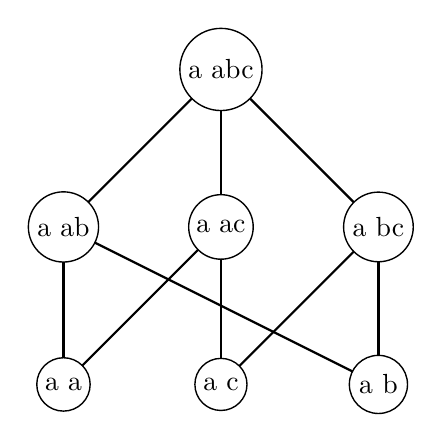
\begin{tikzpicture}
    \SetGraphUnit{2}
    \Vertex{a abc}
    \SO(a abc){a ac}
    \EA(a ac){a bc}
    \WE(a ac){a ab}
    \Edge(a abc)(a ac)
    \Edge(a abc)(a bc)
    \Edge(a abc)(a ab)
    \SO(a ac){a c}
    \EA(a c){a b}
    \WE(a c){a a}
    \Edge(a bc)(a b)
    \Edge(a bc)(a c)
    \Edge(a ac)(a c)
    \Edge(a ac)(a a)
    \Edge(a ab)(a a)
    \Edge(a ab)(a b)
  \end{tikzpicture}
  \caption{Graph of lines dominated by \reline{a~abc}.}
\end{figure}

Note that domination is not the same relation as the subset relation of generated configurations. \reline{a abc ade} generates $[a, b, e]$, while \reline{a a bcde} only generates configurations that are in the former. Yet they are incomparable in terms of domination.

The subset of $A_{1}$ dominated by none is called the \emph{maximal form} of $P_{0}$. Or one could say that the maximal form of $S$ is the Pareto front of \emph{valid} lines with respect to domination, where valid means that a line only generates configurations that $S$ generates.

It seems unlikely that some approximation of the maximal form would be cheaper to compute, as any result of round elimination must include the maximal lines. An approximation would just include some extra lines along with them.

This work's main contribution is a new algorithm for finding the maximal form of $P_{0}$ by combining lines and its proof.

TODO explain proof that sets of configurations and lines are isomorphic

\subsection{Putting it all together}

To perform round elimination, one first finds the maximal form of $P_0$. The new active side, $A_1$, is a version of the maximal form where every set contains a single element, the corresponding set from the maximal form.

The new alphabet, $\Sigma_1$ consists of all symbols found in $A_1$.

The new passive side is built by replacing every set in $A_0$ with the set of all symbols from $\Sigma_1$ that it intersects.

Finally, to make the representation more compact, $\Sigma_1$ is converted from subsets of $\Sigma_0$ to ordinals simply by enumerating the symbols.


\section{Maximization via line combination}\label{nlproof}

In this section I will present a maximization algorithm based on combining lines and prove its correctness. In section~\ref{mechproof}, I will present the corresponding Coq lemmas.

\subsection{Combining lines}

The new maximization algorithm mostly consists of combining lines. Two lines can be \emph{combined} by pairing up their sets and taking the union of one pair and the intersection of the rest.

\begin{figure}[h]
\begin{align*}
  \{I,O\} &\cup \{O\} = \{I, O\} \\
  \{I,O\} &\cap \{I,O\} = \{I, O\} \\
  \{O\} &\cap \{I, O\} = \{O\}
\end{align*}
\caption{one possible way to combine \reline{IO IO O} with itself}
\end{figure}

\begin{theorem}[Combination is sound]
\label{sound}
A combination $C$ of lines $A$ and $B$ only generates configurations present in $A$ or $B$.
\end{theorem}

\begin{proof}
For each configuration $c$ generated by $C$, w.l.o.g.\ suppose the symbol chosen from the union is from $A$. The symbols that come from intersections are in both $A$ and $B$. Thus all symbols in $c$ are from $A$.
\end{proof}

\subsection{Domination relation}

A \emph{maximal line} is a line that no valid line strictly dominates. The \emph{maximal form} is simply a collection of all the maximal lines.

\begin{lemma}
\label{domtrans}
The domination relation is transitive.
\end{lemma}

\begin{proof}
Let line $a$ dominate $b$ and $b$ dominate $c$. Choose some ordering for $b$. Order $a$ so that each of its sets includes $b$'s set. Order $c$ so that each of its sets is included in $b$'s set. As set inclusion is transitive, the corresponding sets of $a$ and $c$ are included in each other.
\end{proof}

\begin{lemma}
The strict domination relation is well-founded.
\end{lemma}

\emph{Well-founded} means that in any set, there is a minimal element. In our case that means that there is a line that doesn't strictly dominate any other line. This property is used later to perform induction on lines.

\begin{proof}
Define the weight of a line as the sum of its sets' cardinalities. Obviously no line can have a negative weight. If a line $a$ strictly dominates line $b$, then the weight of $b$ is less than the weight of $a$, since all of $b$'s sets are subsets of $a$'s and one is a strict subset.

A suitable minimal line for any set is the line with the lowest weight. If there was a line strictly dominated by the lowest-weight line, that line would have even lower weight, which is a contradiction.
\end{proof}

\subsection{Building lines}

A \emph{singleton line} is a line that generates just one configuration. It is the configuration with each symbol wrapped in a set.

\begin{lemma}[Line splitting]
\label{linesplit}
For any non-singleton line $x$ there exist two lines strictly dominated by $x$ that can be combined into $x$.
\end{lemma}

\begin{proof}
Since $x$ is not a singleton line, one of its sets, $S = \{a, b, \dots\}$, must contain multiple elements. Make two lines: one where $S$ is replaced with $S \smallsetminus a$ and another where $S$ is replaced with $S \smallsetminus b$. $(S \smallsetminus a) \cup (S \smallsetminus b) = S$, so $x$ can be built out of them and $x$ strictly dominates them, as they have strictly less symbols in them.
\end{proof}

\begin{theorem}
\label{explode}
Any line can be built by combining singleton lines that it dominates.
\end{theorem}

\begin{proof}
One can perform well-founded induction on lines because the strict domination relation is well-founded. Thus it suffices to show that if all lines strictly dominated by $x$ can be built from dominated singleton lines, $x$ can be, too.

If $x$ is not a singleton line, we can use the line splitting lemma (Lemma \ref{linesplit}) to show that it can be built out of two lines that it strictly dominates. The induction hypothesis tells us that those lines in turn can be built from dominated singleton lines.
\end{proof}

\begin{lemma}[Bigger is better]
\label{biggood}
If lines $a$ and $b$ can be combined into $c$ then $a'$ that dominates $a$ and $b'$ that dominates $b$ can be combined into $c'$ that dominates $c$.
\end{lemma}

It is clear that if $a'$ and $b'$ are combined in the same fashion as $a$ and $b$, the result cannot contain less symbols.

\begin{theorem}[Combination is complete]
\label{complete}
A line dominating any valid line $x$ can be built by combining input lines.
\end{theorem}

\begin{proof}
According to Theorem \ref{explode} $x$ can be built from singleton lines that it dominates. Those singleton lines are valid as well, since dominated lines generate strictly less configurations. Being valid singletons, they generate one configuration each, which is contained in some input line.

If one combines those input lines instead, the result is a line dominating $x$ according to Lemma \ref{biggood}.
\end{proof}

\begin{corollary}
The maximal lines can be built by combining input lines.
\end{corollary}

\begin{proof}
A line is maximal if no valid line strictly dominates it. Thus a valid line dominating a maximal line must be equal to it. Lines obtained by combining input lines are valid; Theorem \ref{sound} shows that combining does not enable new configurations.
\end{proof}

\subsection{Efficiently finding the maximal lines}

Even if combining lines eventually produces the maximal lines, it may not be an efficient way of finding them. Building a maximal line could require hundreds of combinations!

Define a \emph{missing line} as a valid line dominated by none of the input lines.

\begin{lemma}
\label{biggermissing}
A line that dominates a missing line is also missing.
\end{lemma}

\begin{proof}
Let $a$ and $b$ be any lines such that $b$ dominates $a$ and $a$ is missing. Suppose that $b$ is not missing. Then there is an input line $i$ that dominates $b$. Because the domination relation is transitive (Lemma \ref{domtrans}) $i$ dominates $a$ as well, so $a$ is not missing, which is a contradiction.
\end{proof}

\begin{theorem}
\label{justtwo}
If there is a missing line, then some missing line can be obtained by combining two input lines.
\end{theorem}

In other words, we can make progress by simply trying all combinations of two lines.

\begin{proof}
According to Theorem \ref{complete}, there is some way of combining input lines that produces the missing line. Since they are combinations of the input lines, all lines leading up to the missing line are valid due to Theorem \ref{sound}.

By definition a line that is valid but not missing is dominated by some input line. Thus all of them are either missing or dominated by an input line.

Suppose that the lines that combine into the missing line are dominated by input lines. Combining those input lines in the right way yields a line that dominates the missing line according to Lemma \ref{biggood}. Lemma \ref{biggermissing} tells us that bigger line is missing as well.

If one (or both) of the lines are missing, recurse into the missing line. There will be a pair of non-missing lines eventually, as the combination starts with input lines.
\end{proof}

Theorem \ref{justtwo} gives an efficient process for checking maximality: if all ways of combining two lines result in lines dominated by some existing line, then the current set of lines is maximal.

A trivial extension yields an algorithm for finding the maximal form: The input lines start in a todo set and there is an empty done set. As long as there are lines in the todo set, take one of them. If it is dominated by some other line in either set, discard it. Otherwise insert it into the done set and insert all combinations of it and lines in the done set into the todo set.


\section{Type theory as mathematical foundation}

\subsection{Dependent types}\label{dependent}

A dependently typed programming language can express types that depend on values as opposed to simply typed languages, where types and values are entirely separate. Without dependent types, Coq would be useless. For instance, exists quantifiers in Coq create $\Sigma$-types, which do not exist in simply typed languages. Thus it is prudent to study dependent types if one wishes to understand the type theory flavour of proof assistants.

Most programmers are familiar with the notation $e : T$ which is read as expression $e$ has type $T$. This is analogous to set membership in set theory if $T$ is seen as the set of all values that $e$ could have. Types are not sets and don't always behave in the same way but the algebraic operations presented next will look very similar for both. Notably, types don't support union and intersection like sets do.

Types that are checked at runtime, found for example in Python are not the same thing. In Python, the same expression can have a different type on different runs; in statically typed languages every expression has just one type, which can be computed without running the program. In dependently typed languages the parts of the program that appear in types may have to be evaluated during type checking.

\subsubsection{Type algebra}

The unit type $1$ is a type with only one inhabitant, commonly denoted as the empty tuple $()$. The type $0$ is a type that no value has. It should not be confused with \textbf{void} in C, which is actually $1$. If a function's return type is $0$, the function must never return, as it is impossible to construct a value of type $0$.

Values of a product type $A \times B$ consist of an $a : A$ followed by a $b : B$. The cartesian product is the corresponding set operation. Many programming languages have a tuple type, which is a pure product type. Record or struct types are common named variants of product types. In most cases, they could be replaced with tuples; the names are only for making them more readable.

Values of a sum type $A + B$ are either of type $A$ or of type $B$. The corresponding set operation is the disjoint union. A disjoint union is a union where the elements are augmented with an index indicating the set from which set they originate. In programming, this is known as tagged union. Enumerations are the simplest example; booleans could be written $1 + 1$, though it is more concise to call them $2$. A tagged union with zero variants cannot be constructed so it is $0$. Optionals found in Rust or Scala among others, are of the form $T + 1$. Structurally typed unions, an intermediate between C's wildly unsafe unions and tagged unions is found in gradually typed languages like TypeScript and in the joke language IntercalScript~\cite{ICS}.

Knowing this much type algebra is sufficient to understand why the two kinds of dependent types are called $\Pi$ and $\Sigma$-types but I'll go on to show that types equipped with the previously defined sum and product form a semiring to highlight that there truly is an algebra of types.

I have many times found myself wondering if I should write a data structure $A \times (B + C)$ or $(A \times B) + (A \times C)$ when it isn't entirely clear if $A$ really represents the same thing in both cases. I am not aware of any programming language where such \emph{isomorphic types} can be used interchangeably. Incidentally, in Coq $((1, 2), 3)$ is equal to $(1, 2, 3)$ but $(1, (2, 3))$ has a different type.

\begin{theorem}
  The operations $+$ and $\times$ form a semiring on the isomorphism classes of types.
\end{theorem}

\begin{proof}
  It is clear that $+$ is associative and commutative. Its neutral element is $0$; a variant holding zero will never be constructed, so an added $0$ does nothing.

  We can translate between $((a, b), c)$ and $(a, (b, c))$, so $\times$ is associative. The neutral element of $\times$ is $1$, as it doesn't add any information, like struct padding in C.

  Distributivity: $A \times (B + C) \cong (A \times B) + (A \times C)$. As discussed earlier, $0$ is impossible to construct, so a tuple containing it is, too: $A \times 0 = 0$.
\end{proof}

Finding an isomorphism, a one-to-one mapping, is equivalent to showing that two sets have the same cardinality, so finite types can be identified by natural numbers. We already saw the types $0$, $1$ and $2$. For finite types, one could just have stated that $|A + B| = |A| + |B|$ and $|A \times B| = |A||B|$ and used the fact that natural numbers form a semiring. The problem with non-finite types is that depending on the type system, they may not correspond to ordinals or any other well-known kind of integers.

From the cardinality point of view, it is easy to see that the arrow $\to$ in function types corresponds to exponentiation; a function is just a table of outputs with an entry for each input.
\begin{equation*}
  |A \to B| = |B|^{|A|}
\end{equation*}
A table of things of type $T$ is just $T$ raised to some power.

Inductive types have interesting equations, for example
\begin{align*}
  \text{List} &= 1 + (A \times A) + (A \times A \times A) + \ldots
\end{align*}
is a solution to
\begin{align*}
  \text{List} &= (A \times \text{List}) + 1
\end{align*}
which is the typical definition of a list in functional programming languages. Conor McBride~\cite{typeDerivative} has even shown that the partial derivative of a type is a data structure representing an in-progress traversal of it.

\subsubsection{Dependent functions}

A $\Pi$-type is a type that depends on the value passed in. For example, ordinarily it would be impossible to write a function that sums all entries in a tuple because tuples of different lengths have different types. Using a $\Pi$-type, the function could have the type $\Pi_{n : \mathbb N}~\mathbb N^n \to \mathbb N$.

In dependently typed programming languages, $\Pi$-types typically look like ordinary functions. For example, the previous example can be written in Coq as
\begin{minted}{Coq}
Fixpoint ntuple n T : Type :=
  match n with
  | 0 => T
  | S n' => ntuple n' T * T
  end.

Notation "T ^ n" := (ntuple n T).

Fixpoint sumt (n : nat) (nats : nat^n) :=
  match n return nat^n -> nat with
  | 0 => fun x => x
  | S n => fun a => let (r, x) := a in sumt n r + x
  end nats.
\end{minted}

The universal quantifier \icoq{forall x : T, P x} is another way to write a $\Pi$-type in Coq.

Why is it called a $\Pi$-type? A type $\Pi_{e:T}~D(e)$ could be seen as the image $D[T]$, which contains the value of $D$ for all values that $e$ can have. That image is a product type, which is denoted with $\Pi$ just like products on numbers.

\subsubsection{Dependent pairs}

If the naming of $\Sigma$-types follows the same pattern as the naming of $\Pi$-types, then $E = \Sigma_{e:T}~D(e)$ is the sum of the image $D[T]$. And it is! A value of type $E$ contains just one of the values that $D(e)$ can have. And we know the value of $e$, too, because $+$ is a disjoint union.

In dependently typed programming languages, $\Sigma$-types often look like ordinary data structures. One could add a data structure that stores a tuple of arbitrary length to the previous example:
\begin{minted}{Coq}
  Inductive tlist T := make_tlist (n : nat) (l : T^n).
\end{minted}
Explicit $\Sigma$-types are called dependent pairs by programmers. The Coq standard library defines syntax for dependent pairs that allows writing \icoq{tlist} as
\begin{minted}{Coq}
  Definition tlist2 T := { n & T^n }.
\end{minted}

Viewed as a proposition, $\Sigma_{x:T}~P(x)$ corresponds to $\exists x : P(x)$.

\subsubsection{Other exotic types}

$\Sigma$ and $\Pi$-types are not the only kinds of new types that can exist in dependent type theories.~\cite{hofmann1997syntax} For instance Rathjen~\cite{griffor1994strength} has shown that extending Martin-Löf type theory with well-founded tree types makes it a significantly stronger proof system.

Coq's \icoq{Inductive} definitions can be used to define many kinds of dependent types but not all of them; for example higher inductive types are not supported.

\subsubsection{Universes}

TODO

\subsection{Why Coq}

When I started this project, I chose Coq simply because it is very mature and I knew it to be powerful enough. I now know that type theory based proof assistants like Coq are especially suited to this kind of task because they are capable of \emph{reflection}.

Reflection means that one is allowed to prove something by writing a program that checks it, proving that program correct and then using the program in a proof. The key thing that enables reflection in Coq is that its language Gallina is both a programming language and a logic at the same time.

On the flip side, because of Coq's complexity, there are only relatively weak automatic theorem provers for it.

Certified Programming with Dependent Types~\cite{CPDT} has a chapter that goes through progressively more complicated uses of reflection.

To verify a program in a proof assistant that does not support programming, one has to generate lemmas from the source code that is being verified. The seL4 microkernel~\cite{sel4} has been developed in that fashion, for example. That makes sense because high performance and low level access to hardware is vital when implementing an operating system.

Besides, round elimination is commonly used as a subroutine in proofs, while operating systems are not. Embedding round elimination in Coq makes it possible to prove whole reasoning chains. A verified implementation of round elimination by itself doesn't prevent users from giving it the wrong input.

\subsection{Coq Primer (This info will be spread throughout the discussion of the proof)}

\begin{listing}[h]
\begin{minted}{Coq}
Lemma tnth_zip n S T (a : n.-tuple T) (b : n.-tuple S) i :
  tnth (zip_tuple a b) i = (tnth a i, tnth b i).
\end{minted}
\caption{A very simple utility lemma which states that zipping two arrays of the same length and taking the $i$th item produces a tuple with the $i$th item of the first array and the $i$th item of the second list.}
\end{listing}

Lemmas in Coq are types. Constructing any value of type T proves the lemma T.

In Coq it is customary not to assume the law of excluded middle $\forall a : a \lor \lnot a$. This has little effect on the proof at hand, as it is about finite objects. For those a = b is equivalent to a == b and the latter is always true or false, as it can be computed.


\section{Mechanized proof}\label{mechproof}

\begin{listing}[h]
\begin{minted}{Coq}
Theorem is_maximal_form_works :
  is_maximal_form <->
  (∀ x : line, nonzero x -> [exists y in input, perm_eq x y] <-> maximal x).
\end{minted}
\caption{The final theorem that states that \icoq{is_maximal_form} returns true only iff the input consists of the maximal lines.}
\end{listing}

I have formalized the proof presented in Section~\ref{nlproof} and an implementation of maximality checking in Coq. I've written a proof of that implementation's correctness. The proofs involve many boring details, which this thesis does not cover. However, I will show examples of the most important proof techniques used.

This section is written for a reader that has some familiarity with statically typed functional programming but hasn't used Coq. I would encourage readers that have already written some mechanized proofs of their own to study the proof's source code~\cite{source_code} along with the natural language proof (Section~\ref{nlproof}) that closely follows it.

\subsection{Constants and variables}

\begin{listing}[h]
\begin{minted}{Coq}
Variable alphabet_size: nat.
Definition color := 'I_alphabet_size.
Variable delta_minus_one: nat.
Definition Δ := delta_minus_one.+1.

Definition nline n := n.-tuple {set color}.
Notation "n .-line" := (nline n) (at level 30, no associativity).
Definition line := Δ.-line.
Definition configuration := Δ.-tuple color.
\end{minted}
\caption{Definition of lines and configurations used throughout the proof.}
\end{listing}

Variables like \icoq{alphabet_size} automatically become arguments of any function that uses them in Coq. They are very convenient here, as I would otherwise have to explicitly make many lemmas depend on the alphabet size and $\Delta$.

I use \icoq{delta_minus_one} to ensure that $\Delta$ is positive. That way I do not need to deal with the uninteresting case where vertices are not connected at all. I could instead add \icoq{Variable nonzero_delta := Δ <> 0} but then I would have to explicitly use it every time to eliminate the zero case.

\begin{listing}[h]
\begin{minted}{Coq}
Definition contains_unpermuted (cl: configuration) (l: line) : bool :=
  all2 (λ c (s : {set color}), c \in s) cl l.

Definition contains (cl : configuration) (line : line) : bool :=
  [exists (p : configuration | perm_eq p cl), contains_unpermuted p line].

Notation "a ∈ L" := (contains a L) (at level 50, no associativity).
\end{minted}
\caption{Lines are represented as tuples, so their lack of order is simulated, typically by operating on some permutation instead of the actual line.}
\end{listing}

\subsection{Combining lines}

My new maximization algorithm mostly consists of combining lines. Two lines can be combined by pairing up their sets and taking the union of one pair and the intersection of the rest.

\begin{minted}{Coq}
Definition combine m (n := m.+1) (a : n.-line) (b : n.-line) : n.-line :=
  [tuple of (thead a) :|: (thead b)
  :: map (λ ab, ab.1 :&: ab.2) (zip (behead a) (behead b))
  ].

Definition combination_of (a b c : line) :=
  ∃ (a' b' c' : line),
    perm_eq a' a ∧ perm_eq b' b ∧ perm_eq c' c ∧ combine a' b' = c'.

Theorem combination_is_sound (a b c : line) col :
  combination_of a b c -> col ∈ c -> col ∈ a ∨ col ∈ b.
\end{minted}

Proof: For each configuration \icoq{col} in \icoq{c}, wlog. suppose the symbol that comes from the union is from \icoq{a}. The symbols that come from intersections are in both \icoq{a} and \icoq{b}. Thus all symbols in \icoq{c} are from \icoq{a}.

\subsection{Domination relation}

\begin{minted}{Coq}
Definition dominates {n} (b a : n.-line) :=
  [exists a' : n.-line, exists b' : n.-line, perm_eq a a' && perm_eq b b' &&
    all2 (λ x y : {set color}, x \subset y) a' b'].
Notation "a ⊆ b" := (dominates b a) (at level 50, no associativity).
Notation "a ⊈ b" := (~~ dominates b a) (at level 50, no associativity).
Definition strictly_dominates {n} (b a : n.-line) := (a ⊆ b) && (b ⊈ a).
Notation "a ⊂ b" := (strictly_dominates b a) (at level 50, no associativity).
\end{minted}

The strict version of the domination relation is well-founded.

\begin{minted}{Coq}
Definition strictly_dominated (a b : line) := strictly_dominates b a.

Lemma strictly_dominated_wf : well_founded strictly_dominated.
\end{minted}

\section{Performance}

Maximization is the most expensive part of the original Round Eliminator's algorithm. Maximization via line combination is orders of magnitude faster in practice and is resistant to some pathological inputs but it remains the most computationally expensive part of round elimination. % TODO add to abstract maybe?

Evaluating the performance of maximization is difficult, as its output can be exponentially larger than its input. However, there is no known algorithm for checking maximality that is more efficient than performing maximization. Therefore I will compare different algorithms' performance on the decision problem of finding out whether a set of lines is maximal or not.

\subsection{Time complexity of the best previously known algorithm}

The maximization algorithm previously used in Round Eliminator relies on a procedure that transforms a maximal form into a maximal form with one configuration removed. If every configuration was valid, the maximal form would be a single line that generates every configuration, so that line is the starting point. Then each invalid configuration is removed one by one.

The algorithm sees all permutations of a line as separate lines and deduplicates only at the end. I will refer to them as lines and configurations in this description even though I mean their ordered counterparts.

To remove an invalid configuration from a line, the line is split into $\Delta$ different versions that cannot produce the invalid configuration because one of the symbols in the configuration has been removed from each.

The algorithm computes the set of invalid configurations by filtering all $|\Sigma|^{\Delta}$ possible configurations. It produces $\Delta!$ permutations of the output lines before the removal of permutations.

After removing each configuration, dominated lines are discarded with an $O(\Delta n^2)$ pass.

It is unclear how exactly the size of the maximal form develops, so the average number of lines is unknown. Assuming that the number of lines grows linearly, the time complexity of checking maximality is $O(|\Sigma|^{\Delta}{(n\Delta!)}^2)$.

There is an adversarial input that defeats this algorithm. Just concatenate multiple copies of an input, renamed so that each has its own disjoint subset of the alphabet. Then the number of valid lines grows linearly with the size of the input but the number of possible configurations grows to the power of the degree.

\subsection{Time complexity of line combination}

To check maximality with the new algorithm, one has to combine every pair of lines in every possible way and compare the results to the original lines.

The lines can be combined in $n^2\Delta!$ different ways. However, most of those ways result in lines that can be discarded because they contain an empty set or because they are dominated by the original lines or some other combination. Computing the combinations is feasible even for large $\Delta$ when the lines contain many duplicated sets because in that case the order of the duplicated elements has no effect on the outcome. This seems to happen often in practice. However, it is an open question if it is possible to design an algoritm that does not have a factorial worst case.

Comparing two lines can be done by building a bipartite graph where each bipartition represents one of the lines and connecting one side's sets to every set on the other side that is included in them. If there is a perfect matching, one line dominates the other. Bipartite perfect matching can be solved in $O(\Delta^{2.5})$ via the Hopcroft-Karp algorithm. In practice it seems that a backtracking search can be faster but that could be asymptotically worse.

The resulting time complexity is $O(n^{3}\Delta!\Delta^{2.5})$. Notably, the size of the alphabet has no effect on running time anymore.

\subsection{In practice}

I and Dennis Olivetti both implemented the new algorithm in the Rust programming language. TODO link to them.

Both implementations compare new lines against other lines originating from the same pair of lines before comparing against the rest. This is worthwhile based on the assumption that many of the new lines are just inferior versions of the best lines of that batch.

Olivetti showed me that maintaining a set of dominated lines and checking new lines against that set before doing any comparisons improves performance by an order of magnitude in practice, which means that at least in the inputs tested, tens of copies of some useless lines are created.

I would have liked to measure the performance of the Coq function \icoq{is_maximal_form} but it turns out that even on the smallest possible input it requires a finite but large amount of memory. The next section explains how that shortcoming could be rectified.


\section{Discussion}

My goal was to build a provably correct version of round elimination while also improving its performance. I chose to focus solely on maximization, as it is the only nontrivial part of round elimination.

The line combination algorithm for maximization delivers on the performance goal and is already in use but the machine-verified procedure for checking maximality needs more work to be of practical use. This section outlines how one could make the maximality checking program practical and how the proof could be extended to cover round elimination or even whole round eliminator sessions.

\subsection{Impractical data structures}

The formalization of round elimination uses many data structures and proofs provided by the Mathematical Components library. However, that library is made with pure mathematics in mind; functions using the data structures aren't meant to be executed.

Let's take the definition of \icoq{n.-tuple}, a fixed size list, as an example. It is simply a wrapper around a list and a proof that the list's length is \icoq{n}.

\subsection{Formalization methods}

A lot of tedium was involved in formalizing the proofs. I was able to prove very quickly that the result of combining two lines doesn't produce any new colorings. Dealing with the ability to shuffle the lines into any order before combining seemed like something that could benefit from existing theories, so I switched to the mathematical components library at that point.

Explain how ssreflect and math-comp relate to each other

An important idea in math-comp is that every proposition is written as a boolean expression and converted into the most suitable form via a reflection view when necessary.~\cite{mathcompbook} This is good because it makes you think about how you want to proceed with the proof instead of just blindly destructing every conjunction and splitting every disjunction. However, often that is precisely what needs to be done and in that case ssreflect only creates more work.

The big upside of converting between booleans and propositions is that booleans are excellent for doing case analysis or even proofs via computation. Suppose we would like to consider cases where a equals b and where it does not separately. Via small-scale reflection we can view their equality as a boolean and perform case analysis on it. In conventional Coq, one would have to write a function for the type of a and b that either returns that its arguments are equal or that they are not. For equality, the standard library defines a tactic \icoq{decide equality} that fills in the body of such a function but that only works for equality.

Tuple pain

Automation doesn't work with ssr pain (especially lia)

Convoy pattern pain. Code doesn't contain match due to math-comp!

\subsection{A verified Round Eliminator}

Distributed algorithms researchers have found lower bounds for the time complexity of problems by making the problem easier by allowing strictly more configurations, performing round elimination on the result, then making it easier again, etc.\ until they arrive at some well-known problem. It can then be argued that the first problem must be at least as hard as the known problem. (TODO cite a nice example. Maybe the case where they managed to synthesize an algorithm while doing this.) Similarly, upper bounds can be proved by making problems harder.

The Round Eliminator software has tools that can be used to quickly perform a series of simplification and round elimination steps. Each one of the tools produces some new problem that has some relationship to the current problem: easier, harder, exactly as hard or exactly one round easier.

\begin{figure}[h]
  \centering
  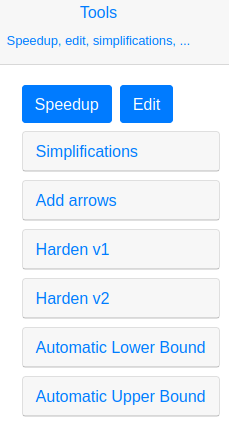
\includegraphics[scale=0.5]{retools}
  \caption{The tools menu of Round Eliminator}
\end{figure}

Each of the tools could be written as a function in Coq, along with proofs of the relationship of their input and output. With a bit of plumbing, these could be used to write reflective proofs like the following:

\begin{minted}{Coq}
Lemma a_harder_than_b : time(A) >= time(B).
  add_line [[C, D], [D, E, F]] A.
  speedup.
  eauto using time_gt_trans.
Qed.
\end{minted}

These could even be automatically generated by Round Eliminator. In cases where Round Eliminator has performed an expensive brute force search, the result of the search can be embedded into the Coq proof in order to avoid running the slower Coq implementations of the tools a lot.

As part of this thesis I have only verified the difficult part of round elimination, maximization. However, I believe that verifying the other tools in Round Eliminator is trivial after formalizing the hardness of problems in some way.

\clearpage
\thesisbibliography{}

\bibliographystyle{plainnat}
\bibliography{correct_round_elimination}

%% Appendices
%% If you don't have appendices, remove \clearpage and \thesisappendix below.
\clearpage
\thesisappendix{}

\section{Esimerkki liitteestä\label{LiiteA}}

Kaavojen numerointi muodostaa liitteissä oman kokonaisuutensa:
\begin{align}
d \wedge A &= F, \label{liitekaava1}\\
d \wedge F &= 0. \label{liitekaava2}
\end{align}

\end{document}
